\documentclass[tikz]{standalone}
\usepackage{pgfplots}
\pgfplotsset{compat=1.15}
\usepackage{mathrsfs}
\usetikzlibrary{arrows,calc}
\usepackage{tkz-euclide}
\pagestyle{empty}

\definecolor{AngleClr}{rgb}{0,0.39215686274509803,0}
\definecolor{ShapeClr}{rgb}{0.6,0.2,0}
\definecolor{KnownLabelClr}{RGB}{65, 143, 20}
\definecolor{UnknownLabelClr}{RGB}{176, 60, 37}

\begin{document}

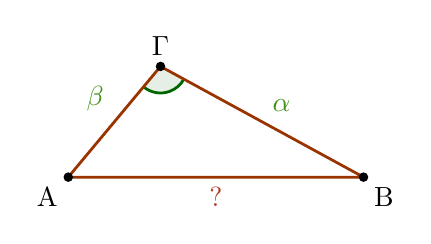
\begin{tikzpicture}[scale=.75]
\tkzSetUpLine[line width=1pt,color=black]
\tkzSetUpPoint[fill=black]

\tkzDefPoints{0/0/A,5/0/B,1.5625/1.875/C}

\tkzFillPolygon[fill=white](A,B,C)

\tkzFillAngle[fill=AngleClr,size=.44,fill opacity=0.1](A,C,B)
\tkzMarkAngle[line width=1pt,size=.45,color=AngleClr](A,C,B)

\tkzDrawPolygon[color=ShapeClr](A,B,C)
\tkzDrawPoints[size=3](A,B,C)
\tkzLabelPoint[below left](A){$\rm A$}
\tkzLabelPoint[below right](B){$\rm B$}
\tkzLabelPoint[above](C){$\rm \Gamma$}

\tkzLabelSegment[above right,KnownLabelClr](B,C){$\alpha$}
\tkzLabelSegment[above left,KnownLabelClr](A,C){$\beta$}
\tkzLabelSegment[UnknownLabelClr](A,B){$?$}
% \tkzMarkSegments[mark=s||,size=2.5](O,A O,B O,C)

\end{tikzpicture}

\end{document}
